\documentclass[]{IEEEtran}

\title{Modeling of a water control system for a tank using SystemC}
\author{Matteo Iervasi - VR439212}

\usepackage{graphicx}
\usepackage[english]{babel}
\usepackage{minted}
\usepackage{tikz}

\begin{document}
\maketitle

\begin{abstract}
This document reports the modeling of a hardware system for controlling the water level of a tank.
It has been modeled using a modular approach, focusing on single parts which has been developed and verified separately,
then merged and tested as a heterogeneous platform.
\end{abstract}


\section{Introduction}
The system has to be able to stabilize the water level of a tank in a precise range through a controller which can adjust
the opening of a valve.
The controller reads the current water level from the tank and sends the valve a command among \texttt{IDLE}, \texttt{OPEN} or \texttt{CLOSE} 
and a threshold, which represents the current maximum aperture of the valve.
The controller encrypts the command using the XTEA protocol, so before going to the valve the command is decrypted by a XTEA decipher.

Given that the system is composed by different parts with different technologies, going with SystemC was a good choice, because of its
ability to represent a model at different levels of abstraction.
Also, the need of having a language able to represent analogue parts brought us using SystemC-AMS, the analogue extension for SystemC.

After separating the various components, each module was developed separately, ensuring it was correct in its behavior.
The digital part, composed of the XTEA module, was developed in four variants, namely RTL and the three TLM styles.
The analogue part, composed of the valve and the water tank was developed using SystemC-AMS, which provides three different
styles for writing analog-mixed signal systems.

I firstly developed the XTEA digital module as a standalone one, then the analogue part, composed of the tank and the valve.
After verifying the correct behavior of the two, I created the heterogeneous system.

\section{Background}
The following technologies were used for the development of the system:
\begin{itemize}
\item \textbf{SystemC}\cite{SystemC}: Standard C++ library for hardware and software platform modeling at different level of abstraction.
\item \textbf{SystemC-AMS} \cite{SystemC-AMS}: Standard C++ library that extends SystemC digital modeling capabilities with analogue modeling.
\end{itemize}
The digital components were described using different levels of abstraction:
\begin{itemize}
    \item \textbf{RTL}: the lowest level of description provided by SystemC, which focuses on signals and registers.
    \item \textbf{TLM}: high level of description which focuses on how modules interact each other.
\end{itemize}
The same for the analogue components:
\begin{itemize}
    \item \textbf{LSF}: stands for \textit{linear signal flow}, describes a continuous non-conservative equation representing the component.
    \item \textbf{TDF}: stands for \textit{timed data flow}, describes a discrete non-conservative equation or function representing the component.
\end{itemize}

\section{Applied methodology}
Following the modular approach, the first component to be developed was the digital XTEA module.

\subsection{XTEA TLM}
The first step involved the development of a TLM description of the XTEA module. Specifically, three variants were coded:
\begin{itemize}
    \item TLM UT (untimed model)
    \item TLM LT (loosely timed model)
    \item TLM AT4 (approximately timed model)
\end{itemize}
Although the final module will only have to decrypt commands, the standalone model is a full implementation of XTEA, which
uses chunks of 128 bits for the key and 64 bits for the text, so a structure is needed. I also need a flag for setting the mode.
In the standalone model of XTEA, I also added a variable for storing the result separately, just for checking the correctness.

The resulting structure was the following:
\begin{minted}{C++}
struct iostruct {
  bool mode;
  sc_uint<32> key[4];
  sc_uint<32> text[2];
  sc_uint<32> result[2];
};
\end{minted}
The module was coded in a single block, using a separate testbench for verifying the correctness, as shown below:
\begin{figure}[H]
\centering
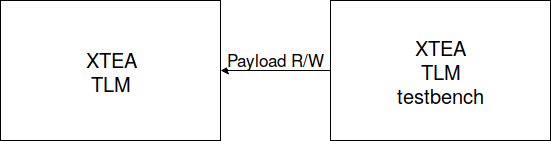
\includegraphics[width=1\linewidth]{figures/xtea_testbench_tlm.png}
\caption{Testbench connection}
\label{fig:xteatestbenchtlm}
\end{figure}

The testbench acts as an initiator communicating with the target (the XTEA module). It calls target's \texttt{b\_transport}, sending it data,
then waits for the answer.
After receiving the answer the initiator can verify the correctness of the data.
Given that I'm using TLM, which focuses on transactions rather than actual implementation, the actual XTEA algorithm is just a C++ function.

Going from untimed TLM representation to a loosely timed one was an easy task. I just added the time notion in the module, simulating the time
spent on computations.

After the LT representation, it was time for the AT4 one. This time things were a bit more complicated. In fact, the AT4 model requires a bidirectional
communication between the initiator and the target that involves 4 steps (that's why it's called ``AT4'').
It was necessary to modify the interface between the initiator and the target so that it was compliant with the style.
You can see the AT4 communication in the following picture:
\begin{figure}[H]
\centering
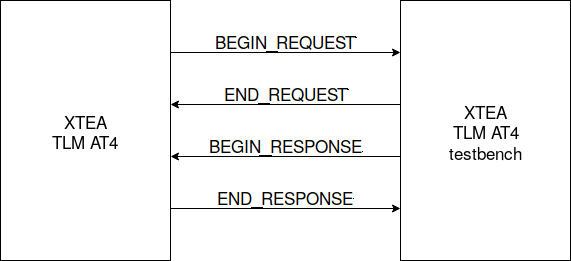
\includegraphics[width=1\linewidth]{figures/xtea_tlm_at4.png}
\caption{The 4 phases of TLM AT4}
\label{fig:xteatlmat4}
\end{figure}
\subsection{XTEA RTL}
The XTEA module was then modeled in RTL. TLM showed us the needed parts with the structure, which now becomes a series of I/O ports.
At this level, I have a clock and a reset that become inputs ports.
In theory, in an RTL implementation one should derive from the C++ algorithm a separation between what has to be a finite state
machine and the datapath, following some design constraints given from the customer (speed vs space constraint as an example).
Here I didn't have any of those, so I decided after taking a look at the XTEA algorithm to just become a datapath.
Obviously if I had to synthesize it on real hardware, it would probably be better to change it, because the area of such
combinational logic would be immense.
The advantage is that the module is very fast and the time to develop it is quite insignificant.
The resulting FSM consists of just two states, \texttt{IDLE} and \texttt{BUSY}.
\begin{center}
    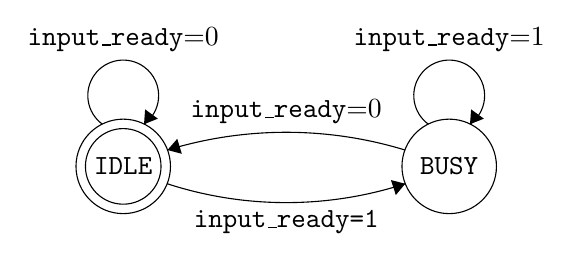
\begin{tikzpicture}[scale=0.2]
    \tikzstyle{every node}+=[inner sep=0pt]
    \draw [black] (26.2,-20.6) circle (3);
    \draw (26.2,-20.6) node {\texttt{IDLE}};
    \draw [black] (26.2,-20.6) circle (2.4);
    \draw [black] (46.9,-20.6) circle (3);
    \draw (46.9,-20.6) node {\texttt{BUSY}};
    \draw [black] (44.111,-21.701) arc (-71.97256:-108.02744:24.433);
    \fill [black] (44.11,-21.7) -- (43.2,-21.47) -- (43.51,-22.42);
    \draw (36.55,-23.4) node [below] {\texttt{input\_ready=1}};
    \draw [black] (24.877,-17.92) arc (234:-54:2.25);
    \draw (26.2,-13.35) node [above] {\texttt{input\_ready}=0};
    \fill [black] (27.52,-17.92) -- (28.4,-17.57) -- (27.59,-16.98);
    \draw [black] (45.577,-17.92) arc (234:-54:2.25);
    \draw (46.9,-13.35) node [above] {\texttt{input\_ready}=1};
    \fill [black] (48.22,-17.92) -- (49.1,-17.57) -- (48.29,-16.98);
    \draw [black] (29.012,-19.559) arc (106.98368:73.01632:25.807);
    \fill [black] (29.01,-19.56) -- (29.92,-19.8) -- (29.63,-18.85);
    \draw (36.55,-17.93) node [above] {\texttt{input\_ready}=0};
    \end{tikzpicture}
\end{center}
When the \texttt{input\_ready} flag is on, it means the module has received the inputs and it can start the computation, so it goes in the \texttt{BUSY}
state. I decided that as long as the flag is on, the FSM stays on \texttt{BUSY} state, so the computation is repeated every time.

The actual RTL implementation was done using an \texttt{SC\_MODULE} with the following I/O ports:
\begin{minted}{C++}
  sc_in_clk clk;
  sc_in<bool> rst;

  sc_in<sc_uint<32>> text_input[2];
  sc_in<sc_uint<32>> key_input[4];

  sc_out<sc_uint<32>> data_output[2];

  sc_in<bool> input_ready;
  sc_in<bool> mode;
\end{minted}
The FSM and the datapath are defined using two separated \texttt{SC\_METHOD}: the FSM is sensible to the \texttt{input\_ready} and the \texttt{mode} ports,
while the datapath is sensible to \texttt{clk} and \texttt{rst}.
The datapath updates the current status and eventually does the computation by calling the \texttt{xtea} method.
The FSM is only responsible for calculating the next state.
The output remains active until \texttt{input\_ready} is active.

The module was then tested with a testbench.

\subsection{Water tank LSF}
After developing the XTEA module, it was time to dive in the AMS part, starting from the water tank, which was suited for LSF style.
\textit{Linear Signal Flow} is a continuous time non conservative mixed signal model. The behavior is defined as relations between variables 
of a set of linear differential algebraic equations. The model is described with a block diagram notation, with signals connecting diagram's blocks.
The blocks (or clusters) are defined in the standard.

The differential equation representing the water tank is
\begin{equation}
\dot{x}=0.6a-0.03x
\end{equation}
The implementation was quite straightforward using standard LSF clusters, connected as shown below:
\begin{figure}[h]
\centering
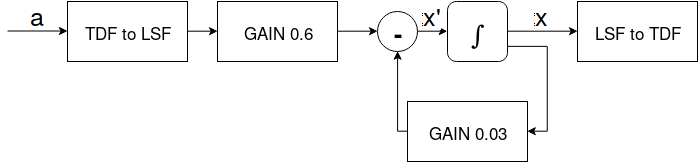
\includegraphics[width=1\linewidth]{figures/LSF.png}
\caption{LSF cluster representation}
\label{fig:lsf}
\end{figure}

The water tank has also a discrete time input port and an output one, for communicating with the valve and the controller.

\subsection{Valve TDF}
After modeling the water tank, I went to the valve. This time, LSF was not very suited, instead I chose to use \textit{Timed Data Flow}.
TDF is a discrete time non conservative mixed signal modeling technique. The process is similar to the RTL one: we define the inputs and the outputs
inside a specific \texttt{SCA\_TDF\_MODULE} plus an internal variable for storing the current valve's aperture.

The module has two specific methods: \texttt{set\_attributes()} and \texttt{processing()}.
With \texttt{set\_attributes()} I can initialize timesteps and the eventual delays, while \texttt{processing()} contains the method executed at every timestep,
so it does the actual work.

Valve's behavior can be expressed as following:
\begin{itemize}
    \item On \texttt{IDLE}:\\
    Do nothing
    \item On \texttt{OPEN}:\\
    $a=a+0.25t$ where $a$ is the aperture and $t$ the timestep
    \item On \texttt{CLOSE}:\\
    $a=a-0.25t$ where $a$ is the aperture and $t$ the timestep
\end{itemize}

\subsection{Controller TDF}
After developing the water tank and the valve, I needed to test the correct behavior. Though the final project requires a TLM controller, I developed a TDF controller
for the standalone AMS project.
The development process was very similar to the one of the valve: the controller periodically reads the water level from the tank, and send a command to the valve, together
with the valve maximum aperture threshold.

\subsection{Heterogeneous platform}
After ensuring everything was behaving correctly, it was time for making the modules work together.
The first problem was that for letting the components communicate each other, I needed transactors.
They are sort of ``translators'' that enables us to make different modules communicate (like a digital RTL module with an AMS one).
Using transactors comes with a drawback: it makes the simulation slower, that's why I had to decrease the controller speed from 5 sec to 2.

Needed transactor were:
\begin{itemize}
    \item \textbf{TLM-RTL}:\\
    SystemC TLM module with the same number output ports as the RTL module's input ports.
    When the \texttt{b\_transport()} function is called values are written.
    \item \textbf{RTL-TLM}:\\
    Module with a looping \texttt{SC\_THREAD}. The TLM controller of the heterogeneous platform is modeled this way.
    \item \textbf{RTL-AMS/AMS-RTL}:\\
    An AMS module that uses \texttt{sca tdf::sca de} ports for converting RTL values to AMS and vice-versa.
\end{itemize}

Picture \ref{fig:system} shows how the heterogeneous platform is built.

After coding the transactors, it was just a matter of testing and parameter tuning.
One notable thing is the valve threshold which, being a real value, was passed directly to the valve instead of being crypted with XTEA,
because it would have been difficult otherwise.

\section{Results}
For testing the correctness of the system, every module was tested both as a standalone one and as a part of the heterogeneous platform.
The testbench tried different inputs and checks for the results, measuring times of simulations.
The first tested module was XTEA. The TLM levels were pretty fast and very similar to each other. RTL was slower, but not that much given
the fact I implemented it as pure combinational logic. It can encrypt and decrypt in 2ns, as shown in figure \ref{fig:rtltime}.

After XTEA I tested the AMS module, which required more time on testing and tuning. Figure \ref{fig:watertank_ams} shows the correct
curve of the water level stabilization.

The heterogeneous platform is shown with two different controller timing in figure \ref{fig:watertank_system_2} and \ref{fig:watertank_system_5}.

\section{Conclusion}
Recycling models and using different level of abstraction can be useful for reducing system modeling and verification, and SystemC makes
this straightforward. Also the possibility to test analogue parts before actually synthesizing the digital ones is very useful for having
at least a working prototype of the digital synthesizable part.

\bibliographystyle{IEEEtran}
\bibliography{biblio}

\appendix

\begin{figure*}[bt]
\centering
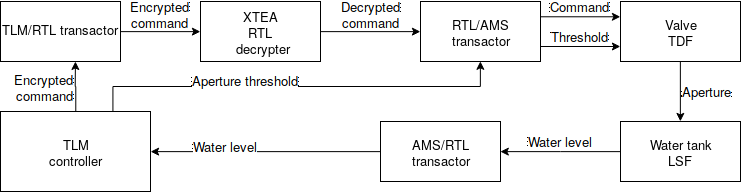
\includegraphics[width=\textwidth]{figures/system.png}
\caption{Heterogeneous platform}
\label{fig:system}
\end{figure*}

\begin{figure}[bt]
\centering
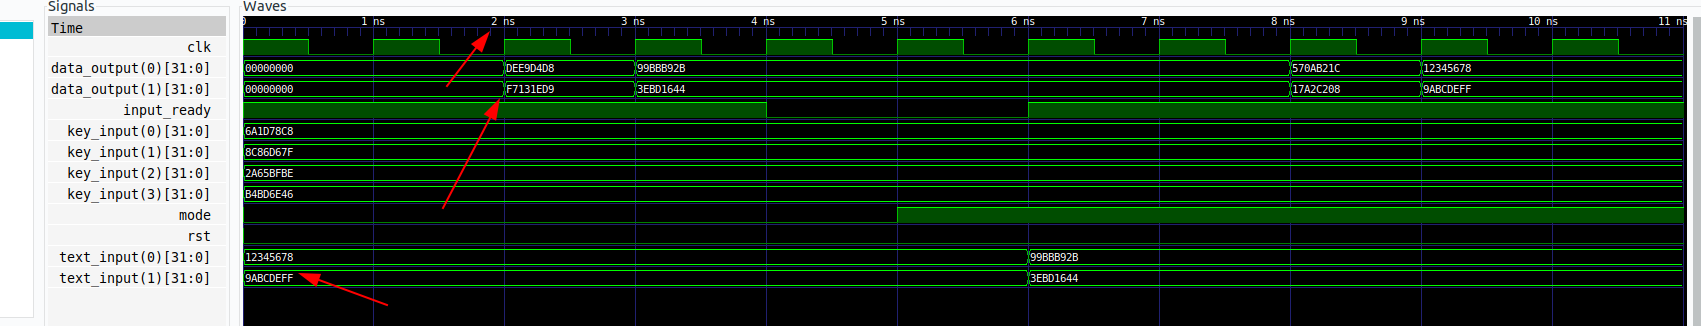
\includegraphics[width=\textwidth]{figures/rtl_time.png}
\caption{RTL times}
\label{fig:rtltime}
\end{figure}

\begin{figure}[bt]
\centering
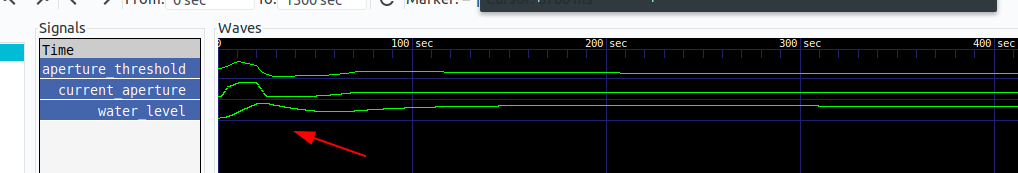
\includegraphics[width=\textwidth]{figures/watertank_ams.png}
\caption{AMS water level stabilization}
\label{fig:watertank_ams}
\end{figure}

\begin{figure}[bt]
\centering
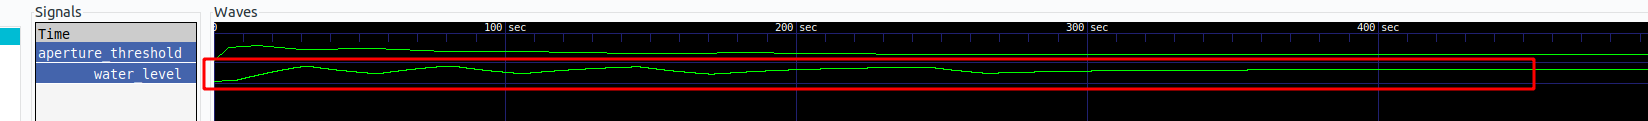
\includegraphics[width=\textwidth]{figures/watertank_system_5.png}
\caption{Water level stabilization}
\label{fig:watertank_system_5}
\end{figure}

\begin{figure}[bt]
\centering
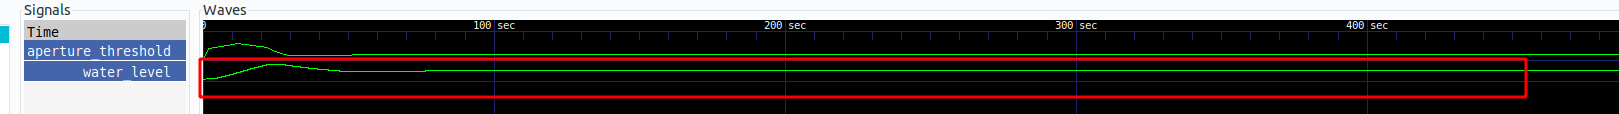
\includegraphics[width=\textwidth]{figures/watertank_system_2.png}
\caption{Water level stabilization}
\label{fig:watertank_system_2}
\end{figure}

\end{document}